\section{Heuristic Redundant Symbols}
\label{sec:hmoves}

The concept of
\textit{heuristic move} is generalized from \textit{default move}.
Let $S$ be the source, $T$ be a target, $F$ be a predefined heuristic function;
$F(S, T)=d$ shows the heuristic move from $S$ to $T$,
and we will put a \heur{} symbol on $T$ if and only if $d$ can be the actual first move. 

Here is a example of $F$:
\begin{itemize}
  \item If $S$ to $T$ needs diagonal moves, then $d$ is the corresponding diagonal move (fig~\ref{hmove1_1});

  \item If $S$ to $T$ may not need any diagonal move, then $d$ is the corresponding straight move (fig~\ref{hmove1_2});

    \begin{figure}[h]
      \centering
      \begin{subfigure}{.35\columnwidth}
      \centering
      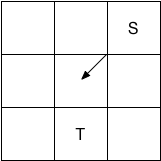
\includegraphics[width=.6\columnwidth]{./hmove1.png}
        \caption{}
        \label{hmove1_1}
      \end{subfigure}%
      \begin{subfigure}{.35\columnwidth}
      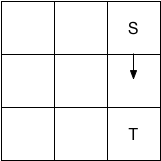
\includegraphics[width=.6\columnwidth]{./hmove1_2.png}
      \centering
        \caption{}
        \label{hmove1_2}
      \end{subfigure}
      \caption{\small Completely obstacle free}
    \end{figure}

  \item $d$ can be adjusted to avoid corner cutting (fig~\ref{hmove2});

    \begin{figure}[h]
      \centering
      \begin{subfigure}{.35\columnwidth}
      \centering
        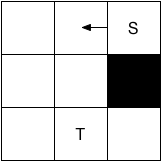
\includegraphics[width=.6\columnwidth]{./hmove2.png}
        \caption{}
        \label{hmove2_1}
      \end{subfigure}%
      \begin{subfigure}{.35\columnwidth}
      \centering
        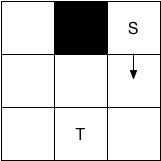
\includegraphics[width=.6\columnwidth]{./hmove2_2.png}
        \caption{}
        \label{hmove2_2}
      \end{subfigure}
      \caption{\small Adjust the heuristic move to avoid cutting corner}
      \label{hmove2}
    \end{figure}

  \item If $d$ is blocked by obstacle(fig~\ref{hmove3}), there are multiple heuristic moves, 
    and we will put the original first move symbol on $T$ to avoid ambiguity.

    \begin{figure}[h]
      \centering
      \begin{subfigure}{.35\columnwidth}
      \centering
        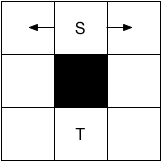
\includegraphics[width=.6\columnwidth]{./hmove3.png}
        \caption{}
        \label{hmove3_1}
      \end{subfigure}%
      \begin{subfigure}{.35\columnwidth}
      \centering
        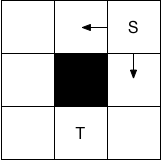
\includegraphics[width=.6\columnwidth]{./hmove3_2.png}
        \caption{}
        \label{hmove3_2}
      \end{subfigure}
      \caption{\small Heuristic move is blocked by obstacle}
      \label{hmove3}
    \end{figure}
  \end{itemize}

Fig~\ref{grid1} shows a visualisation produced by $F$.

\begin{figure}[t]
  \centering
  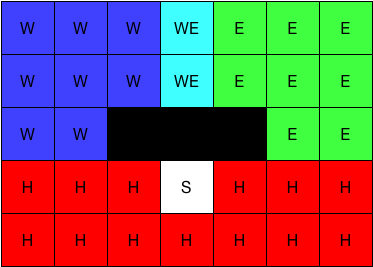
\includegraphics[width=.5\columnwidth]{./grid.png}
  \caption{}
  \label{grid1}
\end{figure}

\section{Improvement}
The heuristic function can be improved by following processes:
\begin{itemize}
  \item When there are multiple heuristic moves, but only one of the heuristic
    move gives the best evaluation (fig~\ref{hmove3_2}), then we can choose such move and put a \heur{}
    symbol there. For example, all blue and green cells in fig~\ref{grid1} can get a \heur{} symbol.
    In other words, the prototype of $F$ has became $F(S, T, tiles_S)$, where
    $tiles_S$ describes the surrounding cell.

  \item When there are multiple heuristic move with same evaluation (fig~\ref{hmove3_1}), we
    can use a predefined ordering (e.g. prefer \textit{W} than \textit{E}) to break the tie. For example, all cyan cells can get
    a \heur{} symbol. In other words, the prototype of $F$ has became $F(S, T, tiles_S, ordering_S)$.

  \item Furthermore, the predefined ordering of each source are independent, so that we can
    find a ordering for each source as long as we can reduce the space cost.

\end{itemize}

After go through above steps, the visualisation becomes fig~\ref{grid2}.

\begin{figure}[t]
  \centering
  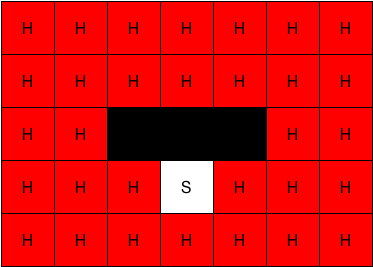
\includegraphics[width=.5\columnwidth]{./grid2.png}
  \caption{}
  \label{grid2}
\end{figure}
